\begin{frame}
  \frametitle{Hybrid $S_N$-Diffusion Method: Literature Review}
  \textbf{Transport-Correction Techniques For Neutron Diffusion-Based Solvers}
  \vspace{.3cm}

  Techniques for augmenting the neutron diffusion method (or equivalent low-order equations) with
  corrections derived from neutron transport:
  \begin{itemize}
    \item Ronen method \cite{ronen_accurate_2004, tomatis_ronen_2021, gross_comprehensive_2023}
    \item Multilevel quasi-diffusion method \cite{goldin_quasi-diffusion_1964, anistratov_computational_2012, tamang_multilevel_2014}
    \item Multischeme transport method \cite{wang_hybrid_2017}
    \item Hybrid transport-diffusion method \cite{anistratov_computational_2012, stehle_hybrid_2014}
  \end{itemize}
  These techniques generally require:
  \begin{itemize}
    \item High-order neutron transport solver
    \item Corrective terms for the neutron diffusion equations
    \item Boundary coupling scheme (for spatial domain decomposition)
  \end{itemize}
\end{frame}

\begin{frame}
  \frametitle{Hybrid $S_N$-Diffusion Method: Literature Review}
  \textbf{The Ronen Method \cite{ronen_accurate_2004, tomatis_ronen_2021, gross_comprehensive_2023}}
  \vspace{.2cm}

  Starting with an initial neutron diffusion flux solution, a transport
  expression is used to iteratively improve the flux solution by updating the
  diffusion coefficients:
  %
  \begin{align}
    D(\vec{r},E) =& -\frac{J_{tr}(\vec{r},E)}{\nabla \phi(\vec{r},E)}
    \label{eq:ronen}
    \shortintertext{where}
    J_{tr} =& \mbox{ transport-derived neutron current.} \nonumber
  \end{align}
  %
  In 1-D slab geometry, the integral expression for calculating the current is:
  %
  \begin{align}
    J(x,E) = \frac{1}{2}\int^a_0 dx'\ &E_2[\tau(x',x,E)sgn(x-x')q_0(x',E) \nonumber \\
    &+\frac{3}{2}\int^a_0dx' \ E_3[\tau(x',x,E)]q_1(x',E)
  \end{align}
  \textbf{Limitation: Demonstrated for 1-D geometries only.}
\end{frame}

%\begin{frame}
%  \frametitle{Hybrid $S_N$-Diffusion Method: Literature Review}
%  \textbf{Transport-Derived Diffusion Closures \cite{pounders_diffusion_2009}}
%  \vspace{.2cm}
%  
%  Pounders \& Rahnema developed two separate methods which also
%  generate space-dependent diffusion coefficients for transport corrections.
%  \vspace{.1cm}
%  \begin{columns}
%    \column[t]{.5\textwidth}
%    \textbf{1) Averaged Eddington Factor Diffusion Theory}
%    %
%    \begin{align}
%      \small
%      E_g(z) =& \frac{\int^1_{-1} \mu^2\psi(z,\mu)d\mu}{\int^1_{-1} \psi(z,\mu)d\mu}
%    \end{align}
%    %
%    \begin{align}
%      \small
%      D^{AEF}_g(z) =& E^i_g\left[\hat{\Sigma}_{t,g}-\sum^G_{g'=1}\hat{\Sigma}^{g'\rightarrow g}_{s1}
%      \frac{\hat{J}_{g'}}{\hat{J}_g}\right]^{-1}
%    \end{align}
%    \hfill
%    \column[t]{.5\textwidth}
%    \textbf{2) High-Order Empirical Diffusion Coefficients}
%    \begin{align}
%      D^i_g =& -\frac{\left(z_{i+1}-z_i\right) \bar{J}_g}{\left[\phi_g(z_{i+1})-\phi_g(z_i)\right]}
%      \label{eq:emp}
%    \end{align}
%  \end{columns}
%  \textbf{Limitation: Both methods require a priori knowledge of the neutron flux and current
%  solution.}
%\end{frame}

\begin{frame}
  \frametitle{Hybrid $S_N$-Diffusion Method: Literature Review}
  \textbf{Multilevel Quasi-Diffusion Method}
  \vspace{.2cm}

  Gol'din originally developed the quasi-diffusion (QD) method as a transport method acceleration
  scheme \cite{goldin_quasi-diffusion_1964}.
  \begin{gather}
    \mbox{\small Zeroth angular moment: } 
    \nabla\cdot J(\vec{r}) + \Sigma_t(\vec{r})\phi(\vec{r}) = \Sigma_{s,0}(\vec{r})\phi(\vec{r}) +
    Q_0(\vec{r}) \label{eq:qd-low-0th} \\
    \mbox{\small First angular moment: }
    \nabla\cdot\left(\vec{\vec{E}}(\vec{r})\phi(\vec{r})\right) + \Sigma_t(\vec{r})J(\vec{r}) =
    \Sigma_{s,1}(\vec{r})J(\vec{r}) + Q_1(\vec{r}) \label{eq:qd-low-1st}
    \shortintertext{\small where}
    \vec{\vec{E}} = \frac{\int_{4\pi}d\hat{\Omega}\ \hat{\Omega}\hat{\Omega}\psi(\vec{r})}{
    \int_{4\pi}d\hat{\Omega}\ \psi(\vec{r})} = \mbox{\small Eddington tensor}.
  \end{gather}
  %
  Gol'din later extended it to a three-level method by deriving effective gray (one-group)
  low-order QD equations \cite{anistratov_solution_1986}.
  \begin{figure}[t]
    \tikzstyle{every node}=[font=\small]
    \centering
    \begin{tikzpicture}
      \node (1) [solver2] {Multigroup high-order transport};
      \node (2) [solver2, right of=1, xshift=3cm] {Multigroup low-order QD};
      \node (3) [solver2, right of=2, xshift=3cm] {Effective low-order transport};
      \draw [arrow] (1.10) -- node[anchor=south, text width=2cm, align=center] {Group\\ Eddington
        and boundary factors} (2.170);
      \draw [arrow] (2.190) -- node[anchor=north, text width=2cm, align=center] {Effective flux
        and precursors} (1.350);
      \draw [arrow] (2.10) -- node[anchor=south, text width=2cm, align=center] {Collapsed Eddington
        and boundary factors} (3.170);
      \draw [arrow] (3.190) -- node[anchor=north, text width=2cm, align=center] {Effective flux
        and precursors} (2.350);
    \end{tikzpicture}
    \caption{Algorithm flowchart for the three-level quasi-diffusion method.}
    \label{fig:algorithm}
  \end{figure}
\end{frame}

\begin{frame}
  \frametitle{Hybrid $S_N$-Diffusion Method: Literature Review}
  \textbf{Multilevel Quasi-Diffusion Method}
  \vspace{.2cm}

  Tamang \& Anistratov applied the QD method to 1-D time-dependent multiphysics neutron transport
  and heat transfer problems by iteratively coupling the gray low-order equations to the heat
  transfer and precursor equations \cite{tamang_multilevel_2014}.
  \vspace{.2cm}

  Reynolds \& Palmer applied the same approach for steady-state simulations of a 2-D axisymmetric,
  two-group MSRE model \cite{reynolds_analysis_2023}.
  %
  \begin{figure}[h]
    \centering
    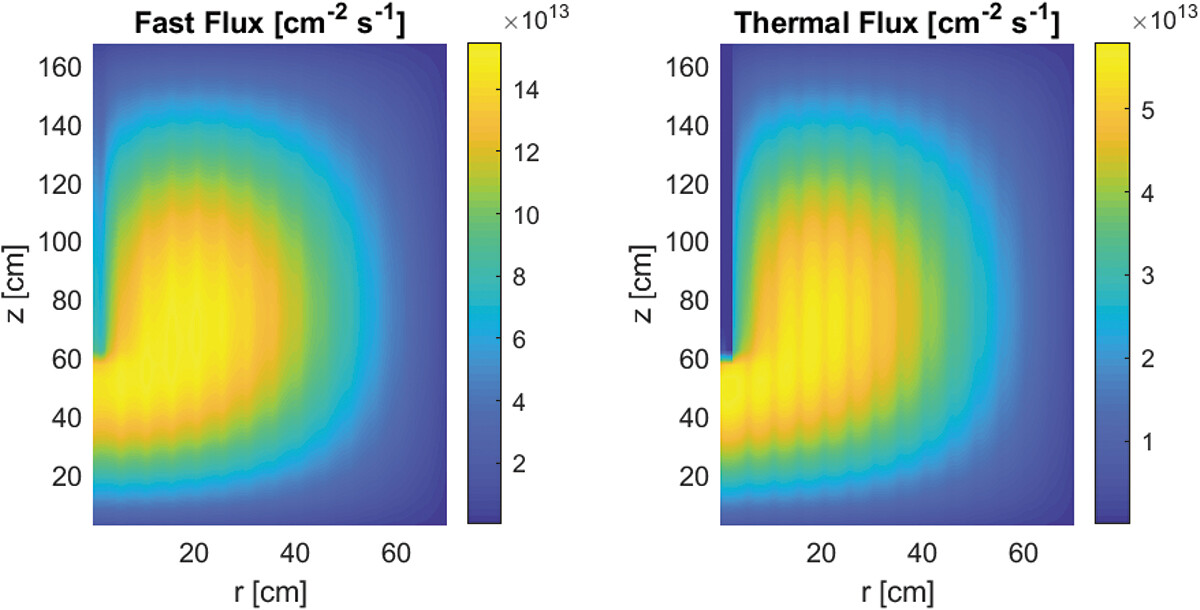
\includegraphics[width=.6\columnwidth]{images/reynolds-flux}
    \caption{Fast and thermal fluxes of the 2-D axisymmetric MSRE model by Reynolds \& Palmer
    \cite{reynolds_analysis_2023}.}
    \label{fig:reynolds-flux}
  \end{figure}
\end{frame}

\begin{frame}
  \frametitle{Hybrid $S_N$-Diffusion Method: Literature Review}
  \textbf{Multischeme Transport Method}
  \vspace{.2cm}

  Implemented in the Griffin reactor physics application. This method involves making predetermined
  domain decompositions to be treated with the $S_N$, $P_N$, or diffusion methods. Adjoining
  subdomains are coupled through the Lagrange multiplier interface condition:
  \begin{gather}
    -\int_S \left[\left(\llbracket\Psi\rrbracket,\Lambda^*\right)_{\Gamma} +
    \left(\llbracket\Psi^*\rrbracket,\Lambda\right)_{\Gamma}\right] d\hat{\Omega}
    \shortintertext{where}
    \begin{align}
      \llbracket\Psi\rrbracket &= \Psi^+ - \Psi^-, 
      \Psi^\pm = \lim_{s\rightarrow 0^+} \Psi(\vec{x}+s\hat{n}), \nonumber \\
      \Lambda &= \mbox{ Lagrange multiplier},
      \Gamma = \mbox{ interface boundary}, \nonumber \\
      \hat{n} &= \mbox{ normal vector at interface boundary}, \nonumber
    \end{align}
  \end{gather}
  or the upwinding method:
  \begin{gather}
    \int_S \left(|\hat{\Omega}\cdot\hat{n}|\llbracket\Psi^*\rrbracket,\Psi^-\right)_{\Gamma^+}
    d\hat{\Omega} -
    \int_S\left(|\hat{\Omega}\cdot\hat{n}|\llbracket\Psi^*\rrbracket,\Psi^+\right)_{\Gamma^-}
    d\hat{\Omega}
  \end{gather}
\end{frame}

\begin{frame}
  \frametitle{Hybrid $S_N$-Diffusion Method: Literature Review}
  \textbf{Hybrid Transport-Diffusion Method}
  \vspace{.2cm}

  Anistratov \& Stehle developed an adaptive domain decomposition scheme using Eddington tensor
  estimates as a metric for deducing whether a region is diffusive or
  transport-like \cite{anistratov_computational_2012, stehle_hybrid_2014}.
  \vspace{.2cm}

  It uses two-level neutronics method based on the Second-Moment method \cite{lewis_comparison_1976}.
  The low-order second-moment equations on the $(s+1)$th iteration are:
  \begin{gather}
    \nabla\cdot J^{(s+1)}+\Sigma_a\phi^{(s+1)} = q, \label{eq:2nd-moment-1} \\
    \frac{1}{3}\nabla\cdot\phi^{(s+1)}+\Sigma_t J^{(s+1)} = \nabla\cdot F^{(s+1/2)}
    \label{eq:2nd-moment-2}
    \shortintertext{where}
    F^{(s+1/2)}_{\alpha\beta} = \int_{4\pi}
    \left(\frac{1}{3}\delta_{\alpha\beta}-\Omega_\alpha\Omega_\beta\right)
    \Psi^{(s+1/2)} d\Omega \label{eq:2nd-moment-3}
  \end{gather}
  %
  The transport subdomains require interface conditions in the form of boundary sources from
  neighboring diffusion subdomains.
\end{frame}

\begin{frame}
  \frametitle{Hybrid $S_N$-Diffusion Method: Literature Review}
  \begin{block}{\textbf{Summary}}
    \begin{itemize}
      \item Corrective terms for the neutron diffusion equations in various forms have been
        effectively applied across various methods.
      \item Domain decomposition is necessary for limiting computational cost in large 3-D reactor
        simulations.
      \item Interface conditions are required when applying domain decomposition to iteratively
        couple the transport and diffusion solvers.
%      \item Demonstrations of the Ronen method are limited to 1-D geometries due to the difficulty of
%        deriving transport operators for complex 2-D and 3-D geometries
    \end{itemize}
  \end{block}
\end{frame}
